\documentclass{article} % Defines the document class
\usepackage{xeCJK}
% Package inclusions go here
\usepackage[utf8]{inputenc} % For UTF-8 encoding
\usepackage[T1]{fontenc} % T1 Font encoding
\usepackage{lmodern} % Modern LaTeX fonts
\usepackage{graphicx} % To include images
\usepackage{indentfirst} % Indent first paragraph after section title
\usepackage{lipsum} % For generating filler text
\usepackage[left=2cm,right=2cm,top=1cm,bottom=2cm]{geometry} % Page margins
% \linespread{1.25}
\usepackage{pdfpages}
\title{评阅后修改情况说明} % Document title
\author{高丁超} % Author name
\date{} % Date
\pagestyle{empty}
\begin{document}

\maketitle % Generates the title
\thispagestyle{empty}

% 本人学位论文在盲审评阅后主要进行了以下修改:
% \section*{表达严谨性}
% 评阅前,本人的学术论文的严谨性存在一些问题,因此进行了如下修改:
% \begin{enumerate}
%     \item 修改前标题使用TDD,表述不清晰。修改后,标题使用TDD全称。
%     \item 修改前在正文中重复介绍TDD全称,写作不规范。修改后仅在第一章第一次出现TDD时介绍TDD全称
%     \item 修改前摘要部分表达生硬,语句不够流畅。修改后对摘要进行了重新表述,突出了主要工作。
%     \item 修改前国外学者人名格式混用,如部分国外学者中间名省略,同时存在译名与原名混用。修改后统一使用国外学者的原名并完整保留中间名。
%     \item 修改前国内学者使用英文拼音,表述不清晰。修改后国内学者全部使用中文原名。
%     \item 修改前专用名词的英文书写格式混乱,写作不规范。修改后所有专有名词出现时,首字母均大写。
%     \item 修改前量子线路的表达不够严谨。修改后对涉及量子线路的表达进行了优化。
%     \item 修改前布尔函数的索引未使用下标,不符合表达习惯。修改后布尔表达式使用下标表示索引。
%     \item 修改前的OpenQASM部分没有给出引用,表达不清晰。修改后增加了参考的论文。
% \end{enumerate}
% \section*{内容完整性}
% \begin{enumerate}
%     \item 修改前部分算法由自然语言给出,同时没有正确性证明和复杂度分析。修改后补充了算法的伪代码和相关分析。
%     \item 修改前论文的总结和展望比较单薄。修改后增加了相关内容。
% \end{enumerate}
% \noindent 申请人签字:
% \hfill[5cm]% Space for signature
% 导师签字:\\[1.5cm]
% \noindent
% \begin{tabular}{p{0.4\linewidth} p{0.4\linewidth}}
%     申请人签字: & \centering 导师签字: \\
% \end{tabular}
% \section*{专家评价意见}
% \setlength{\parindent}{0pt}

% 专家一意见:\\[1.2cm]
% 专家二意见:\\[1.2cm]
% 专家三意见:\\[1.2cm]
% % \begin{tabular}{p{0.4\linewidth} p{0.4\linewidth}}
% %     专家一意见: & \centering 专家二意见:\\
% %     专家三意见: & \\
% % \end{tabular}
% \newpage
% \thispagestyle{empty}

% 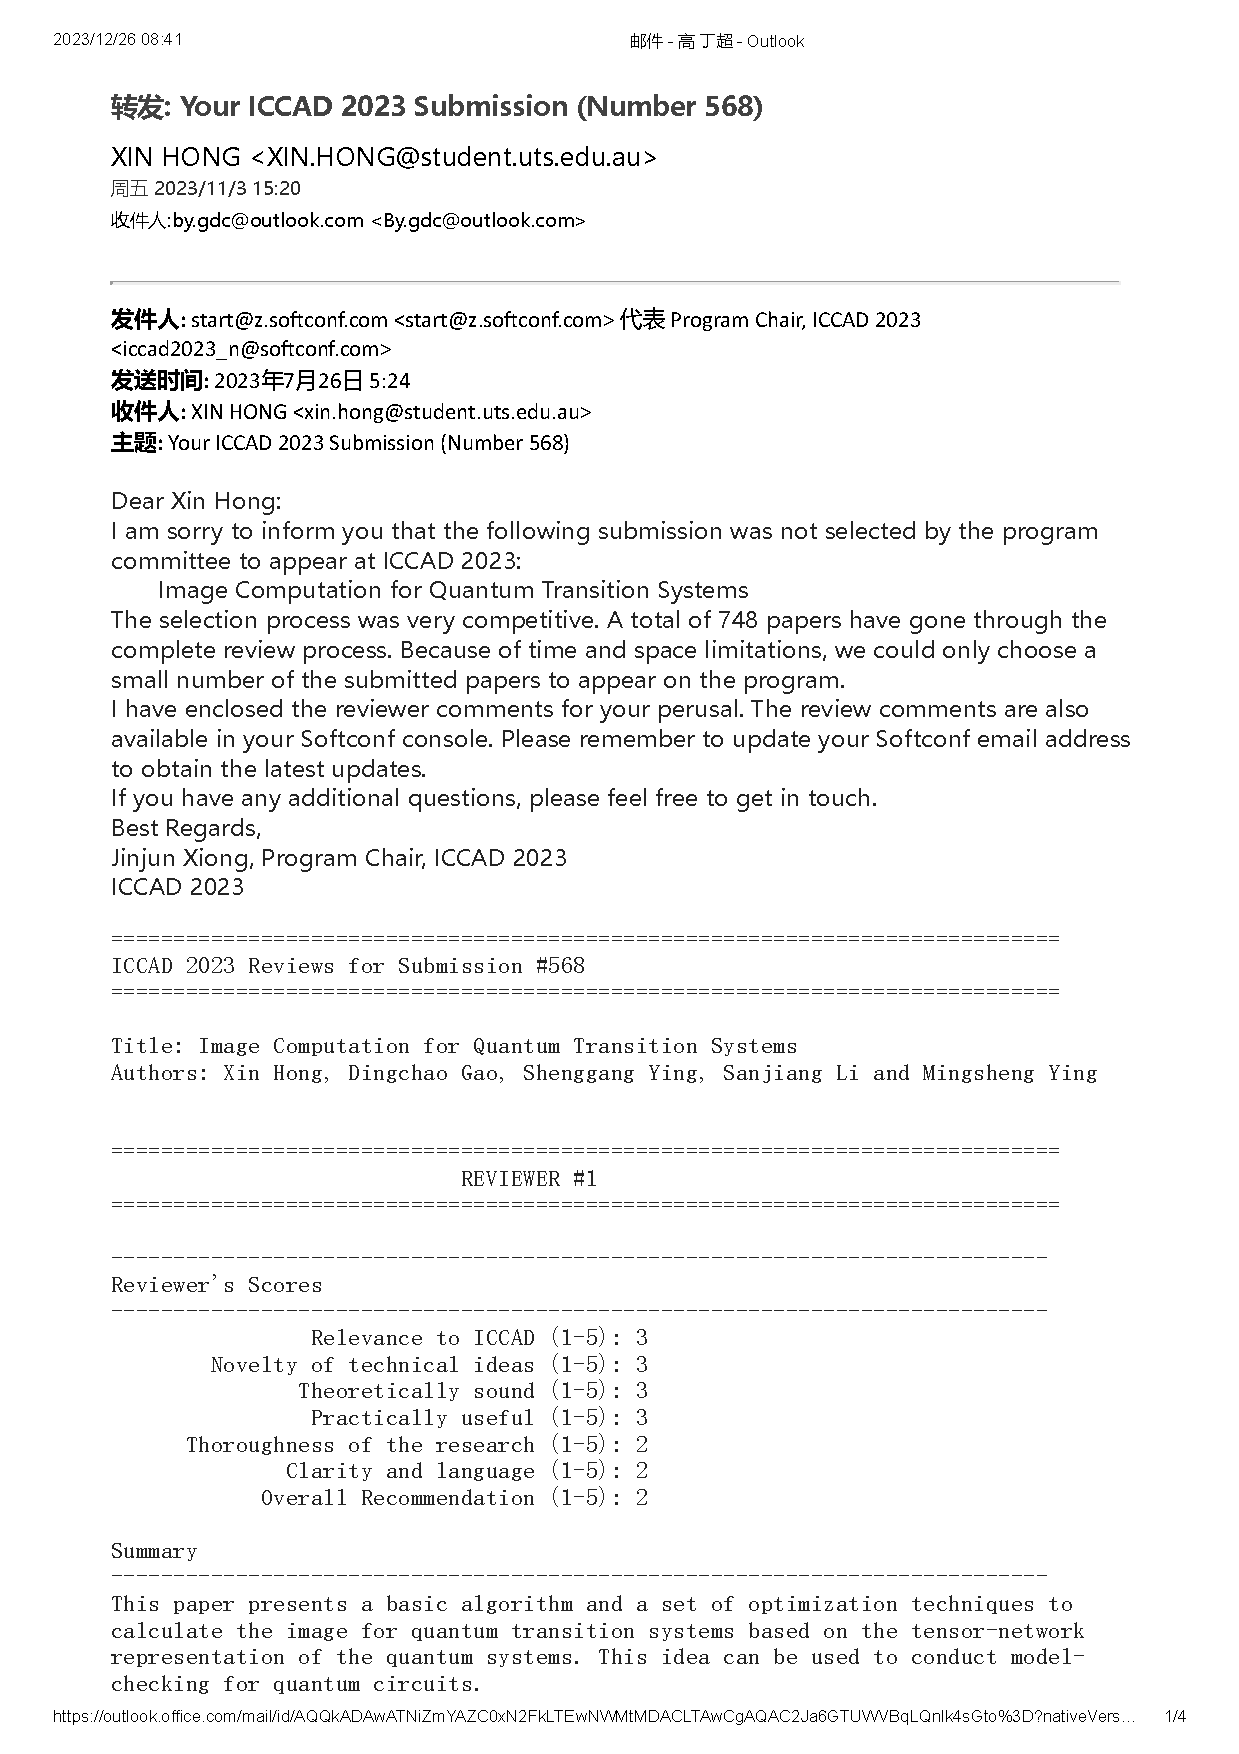
\includepdf[pages=1,scale = 0.8,pagecommand={\section*{附录一ICCAD审稿意见}}]{ICCAD.pdf}
% \includepdf[pages=2-,scale = 0.8]{ICCAD.pdf}
% 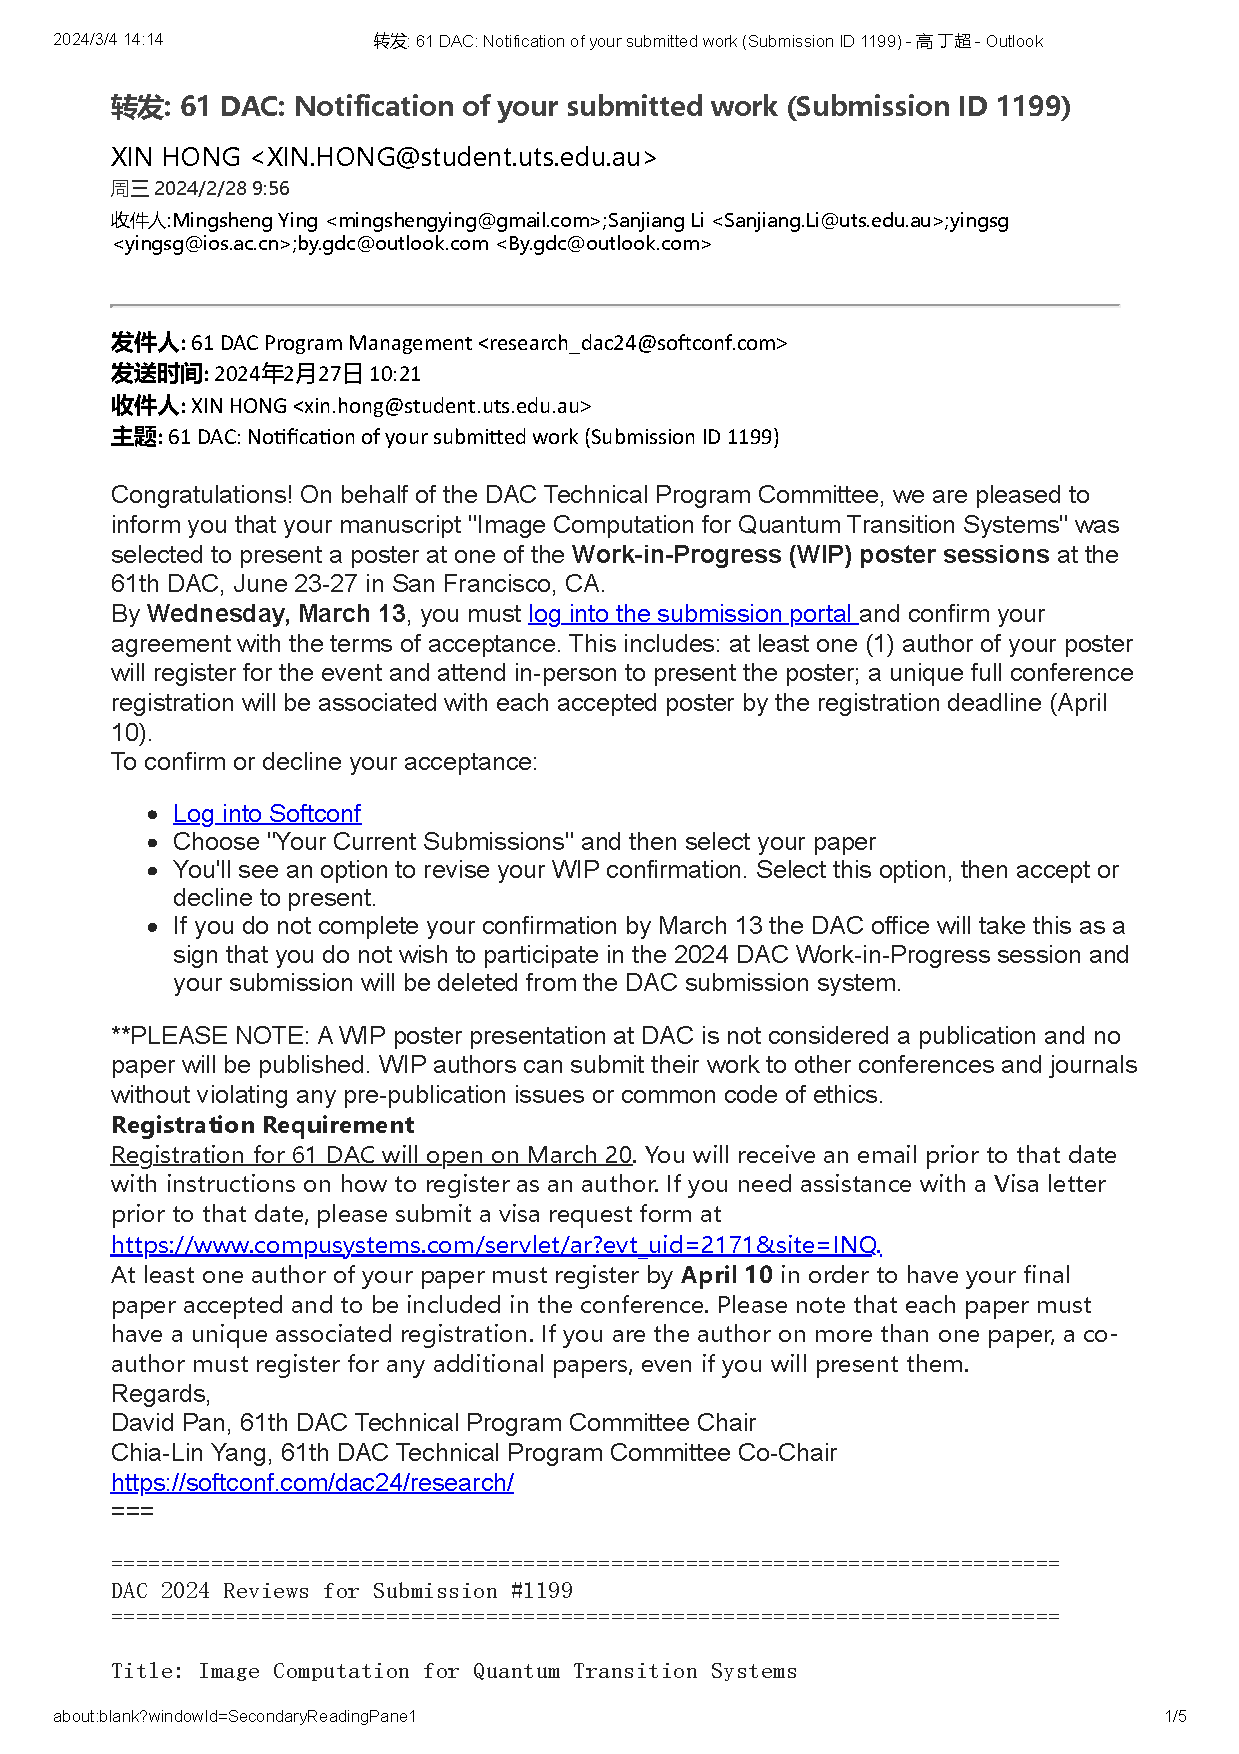
\includepdf[pages=1,scale = 0.8,pagecommand={\section*{附录二DAC审稿意见}}]{DAC.pdf}
% \includepdf[pages=2-,scale = 0.8]{DAC.pdf}

\section*{审稿人一}
\paragraph{学术评语}
本文研究了对一定规模的量子系统进行自动化验证的某些问题,包括将量子线路结构转换为TDD结构,并针对TDD进行模型检测的部分算法。这些对于量子计算算法与线路的模型化、可验证化具有一定的意义,所提方法具有可行性和部分可扩展性,为量子计算机软硬件的形式验证的工具研究提供了有价值的参考。全文格式正确,行文流畅(摘要和有些地方需修改,详见以下),所提理论、模型、公式、算法经验证无重大错误。建议按以下意见对本文进行较系统修改后按期进行答辩。

本文存在存在的部分问题:
\begin{enumerate}
    \item 摘要部分中文较为生硬,语句不够流畅,没有完全凝练全文的内容和主要工作的意义,建议进一步修改并将英文摘要同步进行修改;
    \item 论文中部分文字存在笔误,如大小写(如p.3 QLTL的全称等),国内研究者应写中文名(如应明生等);
    \item 文中一些学术说法不够严谨,如图2-1被描述为制备EPR态的量子线路图,实际上量子线路图必须是描述可逆的量子过程(unitary 过称),2-1只能是量子线路中制备EPR态的一部分量子线路,第四章部分线路图也存在类似问题。
    \item 从第四章开始,作者给出不少算法,多由自然语言描述,应尽量用形式语言如谓词逻辑表达式或者伪代码描述以避免歧义,所有算法应该有正确性证明(大部分算法针对TDD模型,所以无需在量子领域内进行证明,仅针对TDD进行结构归纳等证明即可),应该有时间、空间复杂度和量子资源复杂度分析的过程。
    \item 论文中数处引用了QASM,因为openQASM并非
    学术界通用的标准量子汇编语言,因此应给出QASM的相关specification的引文或者
    预先定义所涉内容。
    \item 部分算法在经典计算机上模拟实现并进行测试,目前已经有
    条件对部分核心算法在实际量子平台上进行小规模测试,未来可考虑进行。
\end{enumerate}
\paragraph{根据意见的修改}
\begin{enumerate}
    \item 已经对摘要进行了重新表述,突出了主要工作。
    \item 已经修改了文中的专有名词描述,并同一了中文学者名的引用。
    \item 已经修改了对量子线路的描述。
    \item 已经补充了第四章中算法的伪代码和相关分析。
    \item 已经增加了openQASM的引用。
    \item 实际量子平台上的规模测试,未来有机会可以实施。
\end{enumerate}
\section*{审稿人二}
\paragraph{学术评语}
论文提出了提出了一种基于张量决策图 (TDD)的量子模型检测新方法,阐述了如何将量子线路转化为 TDD表示,提出了基于 TDD 的量子模型检测算法流程。该研究旨在降低量子模型检测对资源的需求,以扩展量子模型检测的适用范围。论文的选题很好,具有一定的理论意义和应用价值;工作量较充足,难易程度适中,所采用的技术方法可行;论文的结构完整,逻辑清晰,书写规范。作者具备较好的学科理论基础和独立从事科研的能力,可较完整的分析问题和解决问题,达到了硕士学位毕业要求的水平,同意修改后答辩。

存在的问题:
\begin{enumerate}
    \item 文中出现一些语句不通的低级错误,如第4页“更加针对于的,新的验证问题”等。
    \item 文中3.4节的内容是针对模型检测的改进,其中“索引顺序的调整”只分析了研究现状,并没给出解决问题的有效方法,这部分内容出现在文中的意义是什么?其它四项改进方案在4.3节和4.4节有基于实验的分析,那么在3.5节软件系统的实现中,采用了哪个(哪些)方案?为什么?
\end{enumerate}

\paragraph{根据意见的修改与答复}
\begin{enumerate}
    \item 已经修改了病句。
    \item 索引顺序的调整是决策图类型数据结构优化的一个重要方向。3.4节中该部分是为了说明在本次研究中对于索引顺序的处理办法。3.5节的软件系统实现中,实现了论文中讨论的所有方案。这一点已经在论文中重新表述。
\end{enumerate}
\section*{审稿人三}
\paragraph{学术评语}该硕士论文主要借助张量决策图(TDD)去构建量子模型检测可达性分析的方案。该方案的主要思路是根绝张量索引图和实际验证的属性,得到需要收缩的索引和对应索引顺序。该论文围绕几个具体算法进行了实验设计与评估,获得一些基于TDD方法完成可达性分析的优势。该论文有一定创新性,符合硕士答辩要求。

论文还存在一些书写错误以及其他问题,我在此也列举出来:
\begin{enumerate}
    \item 题目中TDD建议直接写作“张量决策图”,正文中可以用TDD表示。并且文中多次重复出现介绍TDD机器全称,例如在第1、3、4页;
    \item 外国人名混用,有的姓名简写而有些未简写。例如在第1章同时出现了诸如E.M.Clarke、Peter Shor、Grover等。同时还同时出现“费曼”的中英文两种写法。建议统一格式;
    \item 中国国内学者建议直接用中文名字,例如文中出现的应明生、冯元等人;
    \item 专有名词第一次出现,后面的英文名词要么全部首字母大写,要么只有第一个首字母大写。例如第三页QLTL和QCTL后面英文书写就不统一,第2章量子计算简介的英文名称出现大量小写字母开头;
    \item 第31页,布尔函数$f(x1,x2,x3,x4)$应为$f(x_1,x_2,x_3,x_4) $(LATEX格式下),类似问题还有很多;
    \item 第5章论文总结与展望内容不够,还需要进一步详实一些。
\end{enumerate}

\paragraph{根据意见的修改}
\begin{enumerate}
    \item 已经参照意见修改标题,并规范了TDD的介绍。
    \item 已经规范了文中的外国学者称呼。
    \item 已经修改了文中国内学者的称呼。
    \item 已经修改了文中专有名词的描述。
    \item 已经规范了文中布尔函数索引下标的使用。
    \item 已经修改对第五章的内容,使得论文总结更加顺畅,同时详实了工作展望。
\end{enumerate}
 \begin{tabular}{p{0.4\linewidth} p{0.4\linewidth}}
    & \\
    & \\
    & \\
	     & \centering 导师签字: \\
\end{tabular}
\end{document}
